\thesischapter{%
    Geometric SMOTE for Imbalanced Datasets with Nominal and Continuous Features
}{%
    Submitted as Joao Fonseca, Fernando Bacao, to a Q1 Journal, 2023
}~\label{chp:gsmotenc}
\graphicspath{{figures/gsmotenc/}}

\begin{adjustwidth}{30pt}{30pt}

    Imbalanced learning can be addressed in 3 different ways: resampling,
    algorithmic modifications and cost-sensitive solutions. Resampling, and
    specifically oversampling, are more general approaches when opposed to
    algorithmic and cost-sensitive methods. Since the proposal of the
    Synthetic Minority Oversampling TEchnique (SMOTE), various SMOTE variants
    and neural network-based oversampling methods have been developed.
    However, the options to oversample datasets with nominal and continuous
    features are limited. We propose Geometric SMOTE for Nominal and
    Continuous features (G-SMOTENC), based on a combination of G-SMOTE and
    SMOTENC. Our method modifies SMOTENC's encoding and generation mechanism
    for nominal features while using G-SMOTE's data selection mechanism to
    determine the center observation and k-nearest neighbors and generation
    mechanism for continuous features. G-SMOTENC's performance is compared
    against SMOTENC's along with two other baseline methods, a
    State-of-the-art oversampling method and no oversampling. The experiment
    was performed over 20 datasets with varying imbalance ratios, number of
    metric and non-metric features and target classes. We found a significant
    improvement in classification performance when using G-SMOTENC as
    the oversampling method. An open-source implementation of G-SMOTENC is
    made available in the Python programming language.

\end{adjustwidth}

\vspace{.5cm}
\textbf{Keywords:} Imbalanced Learning; Oversampling; SMOTE; Data Generation;
Nominal Data

\section{Introduction}~\label{sec:introduction-gsmotenc}

% the problem of imbalanced learning
Various Machine Learning (ML) tasks deal with highly imbalanced datasets, such
as fraud transactions detection, fault detection and medical
diagnosis~\cite{tyagi2020sampling}. In these situations, predicting false
positives is often a more acceptable error, since the class of interest is
usually the minority class~\cite{vuttipittayamongkol2021class}. However, using
standard ML classifiers on imbalanced datasets induces a bias in favor of the
classes with the highest frequency, while limiting the predictive power on
lower frequency classes~\cite{lopez2013insight, das2018handling}. This effect
is known in the ML community as the Imbalanced Learning problem.

% existing approaches to address imbalanced learning
Imbalanced learning involves a dataset with two or more target classes with
varying class frequencies. The minority class is defined as the class with the
least amount of observations and the majority class is the one with the
highest amount of observations~\cite{Kaur2019}. There are three main
approaches to address imbalanced learning~\cite{Fernandez2013}: 

\begin{enumerate}
    \item Cost-sensitive solutions attribute a higher misclassification cost
        to the minority class observations to minimize higher cost errors;
    \item Algorithmic level solutions modify ML classifiers to improve the
        learning of the minority class;
    \item Resampling solutions generate synthetic minority class observations
        and/or remove majority class observations to balance the training
        dataset;
\end{enumerate}

Since it is an external approach to imbalanced learning, the latter method
becomes particularly useful. It dismisses the required domain knowledge to
build a cost matrix and the technical complexity or knowledge to apply an
imbalanced learning-specific classifier. Resampling can be done via
undersampling, oversampling, or hybrid approaches~\cite{tarekegn2021review}. In
this paper, we will focus on oversampling approaches.

% prevalence of nominal features in practical classification settings
The presence of nominal features in imbalanced learning tasks limits the
options available to deal with class imbalance. Even though it is possible to
use encoding methods such as one-hot or ordinal encoding to convert nominal
features into numerical, applying a distance metric on mixed-type datasets is
questionable since the nominal feature values are
unordered~\cite{lumijarvi2004comparison}. In this case, one possible approach
is to use models that can handle different scales (\textit{e.g.}, Decision
Tree). However, this assumption may be limiting since there are few ML
algorithms where this condition is verified. Another possible approach is
transforming the variables to meet scale
assumptions~\cite{lumijarvi2004comparison}. This method was explored in the
algorithm Synthetic Minority Oversampling Technique for Nominal and Continuous
features (SMOTENC)~\cite{Chawla2002} (explained in
Section~\ref{sec:related_work-gsmotenc}).

% why typical methods cannot be used on datasets with mixed data types
In the presence of datasets with mixed data types, using most of the
well-known resampling algorithms becomes unfeasible. This happens because
these methods consider exclusively continuous data; they were not adapted to
also use nominal features. Specifically, since the proposal of SMOTE, various
other SMOTE-variants have been developed to address some of its limitations.
Although, there was not a significant development in research to oversample
datasets with both nominal and continuous features. 

% the proposed method
In this paper, we propose Geometric SMOTE for Nominal and Continuous features
(G-SMOTENC). It generates the continuous feature values of a synthetic
observation within a truncated hyper-spheroid with its nominal feature values
using the most common value of its nearest neighbors. In addition, G-SMOTENC
uses G-SMOTE's data selection strategy and SMOTENC's approach to find the
center observation's nearest neighbors. G-SMOTENC is a generalization of both
SMOTENC and G-SMOTE~\cite{Douzas2019}. With the correct
hyperparameters, our G-SMOTENC implementation can mimic the behavior of SMOTE,
SMOTENC, or G-SMOTE\@. It is available in the
\href{https://github.com/joaopfonseca/ml-research}{open-source Python library
``ML-Research''} and is fully compatible with the Scikit-Learn ecosystem.
These contributions can be summarized as follows:

\begin{enumerate}
    \item We propose G-SMOTENC, an oversampling algorithm for datasets with
        nominal and continuous features;
    \item We test the proposed oversampler using 20 datasets and compare its
        performance to SMOTENC, Random Oversampling, Random Undersampling and
        a State-of-the-art oversampler;
    \item We provide an implementation of G-SMOTENC in the Python programming
        language;
\end{enumerate}

% structure of the paper
The rest of this paper is structured as follows:
Section~\ref{sec:related_work-gsmotenc} describes the related work and its limitations,
Section~\ref{sec:proposed_method-gsmotenc} describes the proposed
method (G-SMOTENC), Section~\ref{sec:methodology-gsmotenc} lays out the methodology
used to test G-SMOTENC, Section~\ref{sec:results_and_discussion-gsmotenc} shows and
discusses the results obtained in the experiment and
Section~\ref{sec:conclusion-gsmotenc} presents the conclusions drawn from this study.


\section{Related Work}~\label{sec:related_work-gsmotenc}

A classification problem contains $n$ classes, having $C_{maj}$ as the set of
majority class observations (\textit{i.e.}, observations belonging to the most
common target class) and $C_{min}$ as the set of minority class observations
(\textit{i.e.}, observations belonging to the least common target class).
Typically, an oversampling algorithm will generate synthetic data in order to
ensure $|C_{min}'|=|C_{maj}|=|C_i|, i \in \{1, \ldots, n\}$.

Since the proposal of SMOTE, other methods modified or extended SMOTE to
improve the quality of the data generated. The process of generating synthetic
data using SMOTE-based algorithms can be divided into two distinct
phases~\cite{fernandez2018smote}:

\begin{enumerate}
    \item Data selection. A synthetic observation, $x^{gen}$, is generated
        based on two existing observations. A SMOTE-based algorithm employs a
        given heuristic to select a non-majority class observation as the
        center observation, $x^c$, and one of its nearest neighbors, $x^{nn}$,
        selected randomly. For the case of SMOTE, $x^c$ is randomly selected
        from each non-majority class.
    \item Data generation. Once $x^c$ and $x^{nn}$ have been selected, $x^{gen}$
        is generated based on a transformation between the two selected
        observations. In the case of SMOTE, this transformation is 
        a linear interpolation between the two observations: $x^{gen} = \alpha x^c
        + (1-\alpha) x^{nn}, \alpha \sim \mathcal{U}(0, 1)$.
\end{enumerate}

Modifications to the SMOTE algorithm can be distinguished according to the
phase where they were applied. This distinction is especially relevant for the
case of oversampling on datasets with mixed data types since it raises the
challenge of calculating meaningful distances and k-nearest neighbors among
observations. For example, State-of-the-art oversampling methods, such as
Borderline-SMOTE~\cite{Han2005}, ADASYN~\cite{HaiboHe2008}, K-means
SMOTE~\cite{Douzas2018} and LR-SMOTE~\cite{liang2020lr} modify the
data selection mechanism and show promising results in imbalanced
learning~\cite{Fonseca2021}. However, these algorithms select $x^c$
using procedures that include calculating each observation's k-nearest
neighbors or clustering methods, which are not prepared to handle nominal
data.

Modifications to SMOTE's generation mechanism are uncommon. A few oversampling
methods, such as Safe-level SMOTE~\cite{bunkhumpornpat2009safe} and
Geometric-SMOTE~\cite{Douzas2019} proposed this type of modification
and have shown promising results~\cite{Douzas2019rs}. However, these
methods are also unable to handle datasets with nominal data. Other
methods attempt to replace the SMOTE data generation mechanism altogether
using different Generative Adversarial Networks (GAN)
architectures~\cite{salazar2021generative, koivu2020synthetic, jo2022obgan}.
Network-based architectures, however, are computationally expensive to train
and sensitive to the training initialization. It is also difficult to ensure a
balanced training of the two networks involved and tuning their
hyperparameters is often challenging or unfeasible~\cite{gonog2019review}. 

As discussed in Section~\ref{sec:introduction-gsmotenc}, research on resampling methods
with mixed data types is scarce. The original paper proposing SMOTE also
proposed SMOTE for Nominal and Continuous (SMOTENC), an adaptation of SMOTE to
handle datasets with nominal and continuous features~\cite{Chawla2002}. To
determine the k-nearest neighbors of $x^c$, the Euclidean distance is modified
to include the median of the standard
deviations of the continuous features for every nominal feature with
different values. Once $x^c$ and $x^{nn}$ are defined,  
the continuous feature values in $x^{gen}$ are generated using the SMOTE generation
mechanism. The nominal features are given the most common values
occurring in the k-nearest neighbors.

Recently, a new SMOTE-based oversampling method for
datasets with mixed data types, SMOTE-ENC~\cite{mukherjee2021smote}, was
proposed. This method modifies the encoding mechanism for nominal features
used in the SMOTENC algorithm to account for nominal features' change of
association with minority classes. The Multivariate Normal Distribution-based
Oversampling for Numerical and Categorical features
(MNDO-NC)~\cite{ambai2019multivariate} uses the original MNDO
method~\cite{ambai2018mndo} along with the SMOTENC encoding mechanism to find
the values of the categorical features for the synthetic observation. However,
the results reported in the paper showed that MNDO-NC was consistently
outperformed by SMOTENC, which led us to discard this approach from further
consideration.

Alternatively to SMOTE-based methods, it is possible to use non-informed over
and undersampling methods for datasets with nominal and continuous features,
specifically Random Oversampling (ROS) and Random Undersampling (RUS). These
methods consist of randomly duplicating minority class observations (in the
case of ROS), which can lead to overfitting~\cite{park2021combined,
batista2004study}, or randomly removing majority class observations (in the
case of RUS), which may lead to underfitting~\cite{bansal2021analysis}.


\section{Proposed Method}~\label{sec:proposed_method-gsmotenc}

We propose G-SMOTENC to oversample imbalanced datasets with both nominal and
continuous features. Our method builds on top of G-SMOTE's selection and
generation mechanisms coupled with a modified version of SMOTENC. It
attributes less importance to the nominal features (relative to the continuous
features) when computing distances among observations compared to SMOTENC.
However, this method can be extended with further modifications to the
nominal data encoding and selection mechanisms in future work. 

Similar to G-SMOTE being an extension of SMOTE, G-SMOTENC is also an extension
of SMOTENC since any method or ML pipeline using the SMOTENC generation
mechanism can replace it with G-SMOTENC without any further modifications. The
proposed method is described in pseudo-code in Algorithm~\ref{alg:gsmotenc}.
The functions $SelectionMechanism$ and $GenerationMechanism$ are described in
Algorithms~\ref{alg:selection} and~\ref{alg:generation}, respectively.

\begin{algorithm}
    \SetKwProg{Fn}{Function}{:}{end}
    \SetKwInput{KwGiven}{Given}
    \caption{G-SMOTENC.}\label{alg:gsmotenc}
    \DontPrintSemicolon%
    
    % START
    \KwGiven{Dataset with binary target classes $C_{min}$ and $C_{maj}$}
    \KwIn{$C_{maj}, C_{min}, \alpha_{sel}, \alpha_{trunc}, \alpha_{def}$}
    \KwOut{$C^{gen}$}

    \Begin{
        $N \leftarrow |C_{maj}| - |C_{min}|$ \\
        $C^{gen} \leftarrow \emptyset$\\
        \While{$|C^{gen}| < N$}{
            $x^c, x^{nn}, X^{nn} \leftarrow SelectionMechanism(C_{maj},
            C_{min}, \alpha_{sel})$\\
            $x^{gen} \leftarrow GenerationMechanism(x^c, x^{nn}, X^{nn},
            \alpha_{trunc}, \alpha_{def})$\\
            $C^{gen} \leftarrow C^{gen} \cup \{x^{gen}\}$
        }
    }
\end{algorithm}

G-SMOTENC's implementation involves additional considerations regarding the
management of the nominal features. During the selection mechanism (identified
as the function $SelectionMechanism$), the nominal features are encoded
using the one-hot encoding technique, while the non-zero constant assumes the
value of the median of the standard deviations of the continuous features in
$C_{min}$, divided by two. This encoding mechanism varies from the one in
SMOTENC in order to attribute less weight to the nominal features relative
to the continuous features.

The selection strategy, $\alpha_{sel}$, as well as $C_{min}$ and $C_{maj}$ are
used to determine a central observation, $x^c$, its nearest neighbors,
$X^{nn}$, and one of its nearest neighbors, $x^{nn} \in X^{nn}$. $X^{nn}$ is
calculated using the euclidean distance and both the continuous and encoded
nominal features. The outcome of this step is dependent on the choice of
$\alpha_{sel}$:

\begin{enumerate}
    \item If $\alpha_{sel} = \mathit{minority}$, $X^{nn}$ will consist of
        $x^c$'s \textit{k}-nearest neighbors within $C_{min}$;
    \item If $\alpha_{sel} = \mathit{majority}$, $X^{nn}$ will consist of
        $x^c$'s nearest neighbor within $C_{maj}$; 
    \item If $\alpha_{sel} = \mathit{combined}$, $X^{nn}$ will consist of the
        union between $x^c$'s \textit{k}-nearest neighbors within $C_{min}$
        and $x^c$'s nearest neighbor within $C_{maj}$, \textit{i.e.},
        $C_{min,k} \cup C_{maj,1}$. In this case, $x^{nn}$ is selected using
        the majority class observation within $X^{nn}$ as well as another
        randomly selected nearest neighbor, such that $x^{nn} =
        argmin(||x^{nn}_{min}-x^c||, ||x^{nn}_{maj}-x^c||)$;
\end{enumerate}

Unlike in the original G-SMOTE generation mechanism, $X^{nn}$ is used in the
to determine the nominal feature values of $x^{gen}$ based on the mode of
these features within $X^{nn}$. G-SMOTENC's generation mechanism (identified
as $GenerationMechanism$) uses two hyperparameters to generate the continuous
features in $x^{gen}$: the truncation factor, $\alpha_{trunc}$, and the
deformation factor, $\alpha_{def}$. They are generated by forming a
hyper-sphere with center $x^c$ and is modified according to the parameters:

\begin{enumerate}

    \item $\alpha_{trunc}$ truncates the hyper-sphere to induce the generation
        of the artificial instance within a subset of the hypersphere. It
        varies between 1 and -1, where 1 would split the generation area in
        half and use the area between $x^c$ and $x^{nn}$, -1 achieves the same
        effect and uses the other semi-hyper-sphere, and 0 applies no
        truncation.

    \item $\alpha_{def}$ deforms the hyper-sphere as shown in
        Figure~\ref{fig:gsmote}. It varies between 0 and 1, where 0 applies no
        deformation and 1 fully deforms the hyper-sphere into a line segment,
        corresponding to $e^{//}$.

\end{enumerate}

Figure~\ref{fig:gsmote} depicts the effect of those hyperparameters in the
data selection and generation phases. For an in-depth explanation of these
hyperparameters, the reader is referred to~\cite{Douzas2019}.

\begin{figure}
	\centering
	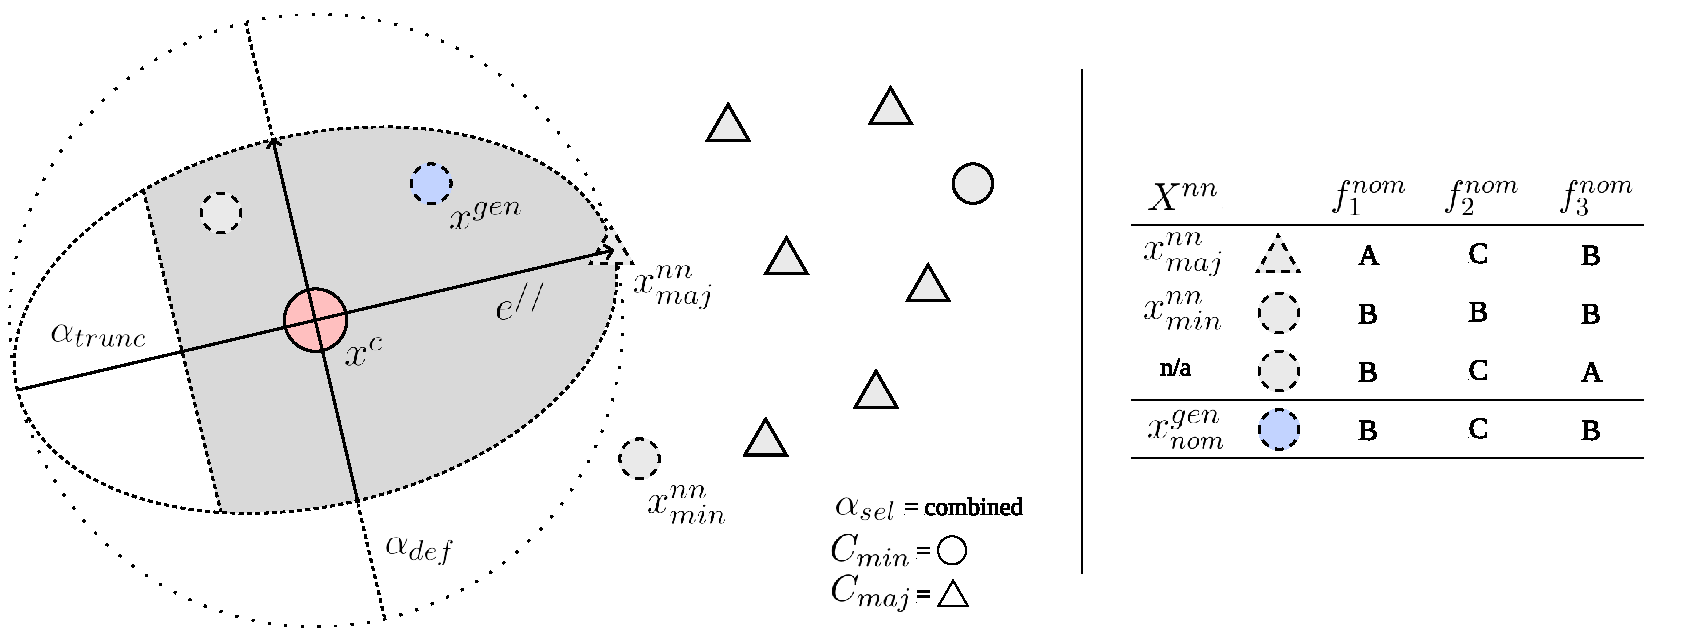
\includegraphics[width=\linewidth]{g-smote}
    \caption[A visual depiction of G-SMOTENC.]{%
        A visual depiction of G-SMOTENC. In this example, $\alpha_{trunc}$ is
        approximately 0.5 and $\alpha_{def}$ is approximately 0.4.
    }~\label{fig:gsmote}
\end{figure}

\subsection{Selection Mechanism}

The data selection mechanism is preceded by the numerical encoding of the
nominal features. It combines the selection mechanisms of SMOTENC and
G-SMOTE, as shown in Algorithm~\ref{alg:selection}. The selection mechanism
inherits the minority, majority, and combined mechanisms proposed in G-SMOTE.
The nominal features in the minority and majority class observations,
$C_{maj}$ and $C_{min}$ are first encoded using a one-hot encoding approach
and replacing the constant 1 with the median of the standard deviations of the
continuous features in $C_{min}$ divided by 2. The nearest-neighbors
($X^{nn}$) of $x^c$ are determined based on $\alpha_{sel}$, which are passed
on to the generation mechanism to determine the nominal features' values of
$x^{gen}$ in the generation mechanism. Simultaneously, $x^{nn}$ is randomly
selected from $X^{nn}$ and will be used to generate $x^{gen}$'s continuous
features' values.


\begin{algorithm}
    \SetKwProg{Fn}{Function}{:}{end}
    \SetKwInput{KwGiven}{Given}
    \caption{G-SMOTENC's selection mechanism.}\label{alg:selection}
    \DontPrintSemicolon%
    
    % START
    \KwIn{$C_{maj}, C_{min}, \alpha_{sel}$}
    \KwOut{$x^c, x^{nn}$, $X^{nn}$}

    \Fn{CatEncoder($C_{maj}$, $C_{min}$)}{
        $S \leftarrow $ Standard deviations of the continuous features in $C_{min}$\\
        $\sigma_{med} \leftarrow median(S)$\\
        \ForAll{$i \in \{maj, min\}$}{
            \ForAll{$f \in C_i^T$}{
                \If{f is nominal}{
                    $f' \leftarrow OneHotEncode(f) \times \sigma_{med} / 2$ \\
                    $C_i' \leftarrow (C_i^T \setminus f)^T$\\
                    $C_i' \leftarrow (C_i'^T \cup f')^T$
                }
            }
        }
        \Return $C_{maj}'$, $C_{min}'$
    }

    \Fn{Surface($\alpha_{sel}$, $x^c$, $C_{maj}$, $C_{min}$)}{
        \If{$\alpha_{sel} = minority$}{
            $x^{nn} \in C_{min, k}$ 
            \tcp*[f]{One of the $k$-nearest neighbors of $x^c$ from
            $C_{min}$}\\
            $X^{nn} \leftarrow C_{min, k}$
        }
        \If{$\alpha_{sel} = majority$}{
            $x^{nn} \in C_{maj, 1}$ 
            \tcp*[f]{Nearest neighbor of $x^c$ from $C_{maj}$}\\
            $X^{nn} \leftarrow C_{maj, 1}$
        }
        \If{$\alpha_{sel}$ = combined}{
            $x^{nn}_{min} \in C_{min, k}$ \\
            $x^{nn}_{maj} \in C_{maj, 1}$ \\
            $x^{nn} \leftarrow argmin(||x^{nn}_{min}-x^c||,
            ||x^{nn}_{maj}-x^c||)$\\
            $X^{nn} \leftarrow C_{min, k} \cup C_{maj, 1}$
        }
        \Return $x^{nn}, X^{nn}$ \tcp*[f]{$X^{nn}$ is the set of $k$-nearest neighbors}\\
    }

    \Begin{
        $C_{maj}', C_{min}' \leftarrow CatEncoder(C_{maj}, C_{min})$ \\
        $x^c \in C_{min}'$ \tcp*[f]{Randomly select $x^c$ from $C_{min}'$}\\
        $x^{nn}, X^{nn} \leftarrow Surface(\alpha_{sel}, x^c, C_{maj}', C_{min}')$\\
        Reverse encoding of nominal features in $x^c$, $x^{nn}$ and $X^{nn}$
    }
\end{algorithm}

\subsection{Generation Mechanism}

G-SMOTENC's generation mechanism is shown in Algorithm~\ref{alg:generation}.
It divides the generation of $x^{gen}$ into two parts: (1) generation of
continuous feature values and (2) generation of nominal feature values.
First, the nominal features from $x^c$ and $x^{nn}$ are discarded. Afterward,
the continuous features are generated using G-SMOTE's generation mechanism;
within a hyper-spheroid defined with $\alpha_{trunc}$ and $\alpha_{def}$,
which allows the non-linear generation of synthetic observations between $x^c$
and $x^{nn}$. Finally, the nominal feature values are generated by the mode of
each feature within the observations in $X^{nn}$.

\begin{algorithm}
    \SetKwInput{KwGiven}{Given}
    \SetKwProg{Fn}{Function}{:}{end}
    \caption{G-SMOTENC's generation mechanism.}\label{alg:generation}
    \DontPrintSemicolon%

    % START
    \KwIn{$x^c, x^{nn}, X^{nn}, \alpha_{trunc}, \alpha_{def}$}
    \KwOut{$x^{gen}$}

    \Fn{Hyperball()}{
        $v_i \sim \mathcal{N}(0, 1)$\\
        $r \sim \mathcal{U}(0, 1)$\\
        $x^{gen} \leftarrow r^{1/p}\frac{(v_1, \ldots, v_p)}{||(v_1, \ldots,
        v_p)||}$\\
        \Return $x^{gen}$
    }

    \Fn{Vectors($x^c, x^{nn}, x^{gen}$)}{
        $e^{//} \leftarrow \frac{x^{nn}-x^c}{||x^{nn}-x^c||}$\\
        $x^{//} \leftarrow (x^{gen} \cdot e^{//})e^{//}$\\
        $x^{\perp} \leftarrow x^{gen} - x^{//}$\\
        \Return $x^{//}, x^{\perp}$
    }

    \Fn{Truncate($x^c, x^{nn}, x^{gen}, x^{//}, \alpha_{trunc}$)}{
        \If{$|\alpha_{trunc} - x^{//}| > 1$}{
            $x^{gen} \leftarrow x^{gen} - 2x^{//}$
        }
        \Return $x^{gen}$
    }

    \Fn{Deform($x^{gen}, x^{\perp}, \alpha_{def}$)}{
        \Return $x^{gen} - \alpha_{def}x^{\perp}$
    }

    \Fn{Translate($x^c, x^{gen}, R$)}{
        \Return $x^c + R x^{gen}$
    }

    \Fn{GenNominal($X^{nn}$)}{
        $x^{gen}_{nom} = \emptyset $\\
        \ForAll{$f \in (X^{nn})^T$}{
            \If{f is nominal}{
                $x^{gen}_{nom} \cup \{mode(f)\}$\tcp*[f]{Ties are decided with
                random selection}\\
            }
        }
        \Return $x^{gen}_{nom}$
    }

    \Begin{
        Discard nominal features from $x^c$ and $x^{nn}$\\
        $x^{gen} \leftarrow Hyperball()$\\
        $x^{//}, x^{\perp} \leftarrow Vectors(x^c, x^{nn}, x^{gen})$\\
        $x^{gen} \leftarrow Truncate(x^c, x^{nn}, x^{gen}, x^{//}, \alpha_{trunc})$\\
        $x^{gen} \leftarrow Deform(x^{gen}, x^{\perp}, \alpha_{def})$\\
        $x^{gen} \leftarrow Translate(x^c, x^{gen},
        ||x^{nn}_{cont}-x^c||)$\\
        $x^{gen}_{nom} \leftarrow GenNominal(X^{nn})$\\
        $x^{gen} \leftarrow x^{gen} \cup x^{gen}_{nom}$
    }

\end{algorithm}


\section{Methodology}~\label{sec:methodology-gsmotenc}

This section describes how the evaluation of G-SMOTENC was performed. We
describe the datasets used in the experiment, their source and preprocessing
steps executed in Section~\ref{sec:experimental_data-gsmotenc}. The resampling and
classification methods used to analyze G-SMOTE's performance are listed in
Section~\ref{sec:ml_algorithms-gsmotenc}. The performance metrics used are defined in
Section~\ref{sec:performance_metrics-gsmotenc}. Finally, the experimental procedure is
described in Section~\ref{sec:experimental_procedure-gsmotenc}.

\subsection{Experimental Data}~\label{sec:experimental_data-gsmotenc}

The datasets used in this experiment were extracted from the
\href{https://archive.ics.uci.edu}{UC Irvine Machine Learning Repository}. All
of the datasets are publicly available and cover a range of different domains.
The criteria to select the datasets ensured that all datasets are imbalanced
and contained non-metric features (\textit{i.e.}, ordinal, nominal or binary).
These datasets are used to show how the performance of different
classifiers varies across over/undersamplers.

All datasets were initially preprocessed manually with minimal manipulations.
We removed features and/or observations with missing values and identified the
non-metric features. The second stage of preprocessing was done
systematically. It starts with the generation of artificially imbalanced
datasets with different Imbalance Ratios ($IR=\frac{|C_{maj}|}{|C_{min}|}$).
For each original dataset, we create its more imbalanced versions at intervals
of 10, while ensuring that $|C_{min}| \ge 15$. The sampling strategy was
determined for class $n \in \{1,\ldots,n,\ldots,m\}$ as a linear interpolation
using $|C_{maj}|$ and $|C_{min}'|=\frac{|C_{maj}|}{IR_{new}}$, as shown in
equation~\ref{eq:sampling}.

\begin{equation}~\label{eq:sampling}
    |C_i|^{imb} =
    \min(\frac{|C_{min}'|-|C_{maj}|}{n-1}.|C_i|+|C_{max}|, |C_i|)
\end{equation}

The new, artificially imbalanced dataset, is formed by sampling observations
without replacement from each $C_i$ such that $C_i' \subseteq C_i , |C_i'| =
|C_i|^{imb}$. The artificially imbalanced datasets are marked with its
imbalance ratio as a suffix in Table~\ref{tbl:datasets_description}.

The datasets (both original and artificially imbalanced versions) are then
filtered to ensure all datasets have a minimum of 500 observations.  The
remaining datasets with a number of observations larger than 5000 are randomly
sampled to match this number of observations. Afterward, we remove target
classes with a frequency lower than 15 observations for each remaining
dataset. Finally, the continuous and discrete features are scaled to the range
$[0,1]$ to ensure a common range between all features. The description of the
resulting datasets is shown in Table~\ref{tbl:datasets_description}.

\begin{longtable}{cccccccc}
\caption[Description of the datasets collected after data preprocessing.]{Description of the datasets collected after data preprocessing. The sampling strategy is similar across datasets. Legend: (IR) Imbalance Ratio}
\label{tbl:datasets_description}\\
\toprule
           Dataset &  Metric &  Non-Metric &  Obs. &  Min. Obs. &  Maj. Obs. &     IR &  Classes \\
\midrule
\endfirsthead
\caption[]{Description of the datasets collected after data preprocessing. The sampling strategy is similar across datasets. Legend: (IR) Imbalance Ratio} \\
\toprule
           Dataset &  Metric &  Non-Metric &  Obs. &  Min. Obs. &  Maj. Obs. &     IR &  Classes \\
\midrule
\endhead
\midrule
\multicolumn{8}{r}{{Continued on next page}} \\
\midrule
\endfoot

\bottomrule
\endlastfoot
           Abalone &       1 &           7 &  4139 &         15 &        689 &  45.93 &       18 \\
             Adult &       8 &           6 &  5000 &       1268 &       3732 &   2.94 &        2 \\
        Adult (10) &       8 &           6 &  5000 &        451 &       4549 &  10.09 &        2 \\
         Annealing &       4 &           6 &   790 &         34 &        608 &  17.88 &        4 \\
            Census &      24 &           7 &  5000 &        337 &       4663 &  13.84 &        2 \\
     Contraceptive &       4 &           5 &  1473 &        333 &        629 &   1.89 &        3 \\
Contraceptive (10) &       4 &           5 &  1036 &         62 &        629 &  10.15 &        3 \\
Contraceptive (20) &       4 &           5 &   990 &         31 &        629 &  20.29 &        3 \\
Contraceptive (31) &       4 &           5 &   973 &         20 &        629 &  31.45 &        3 \\
Contraceptive (41) &       4 &           5 &   966 &         15 &        629 &  41.93 &        3 \\
         Covertype &       2 &          10 &  5000 &         20 &       2449 & 122.45 &        7 \\
   Credit Approval &       9 &           6 &   653 &        296 &        357 &   1.21 &        2 \\
     German Credit &      13 &           7 &  1000 &        300 &        700 &   2.33 &        2 \\
German Credit (10) &      13 &           7 &   770 &         70 &        700 &  10.00 &        2 \\
German Credit (20) &      13 &           7 &   735 &         35 &        700 &  20.00 &        2 \\
German Credit (30) &      13 &           7 &   723 &         23 &        700 &  30.43 &        2 \\
German Credit (41) &      13 &           7 &   717 &         17 &        700 &  41.18 &        2 \\
     Heart Disease &       5 &           5 &   740 &         22 &        357 &  16.23 &        5 \\
Heart Disease (21) &       5 &           5 &   735 &         17 &        357 &  21.00 &        5 \\
\end{longtable}


\subsection{Machine Learning Algorithms}~\label{sec:ml_algorithms-gsmotenc}

The choice of classifiers used in the experimental procedure was based on
their type (tree-based, nearest neighbors-based, linear model and
ensemble-based), popularity and consistency in performance. We used Decision
Tree (DT), a K-Nearest Neighbors (KNN) classifier, a Logistic
Regression (LR) and a Random Forest (RF).

Given the lack of existing oversamplers that address imbalanced learning
problems with mixed data types, the amount of benchmark methods used is also
limited. We used three appropriate, well-known methods and one state-of-the-art
oversampling method: SMOTENC, RUS, ROS and SMOTE-ENC\@. Table~\ref{tbl:grid}
shows the hyperparameters used for the parameter search described in
Section~\ref{sec:experimental_procedure-gsmotenc}.

\begin{table}[ht]
	\centering
    \caption{\label{tbl:grid}
        Hyperparameter definition for the classifiers and resamplers used in
        the experiment.
    }
	\begin{tabular}{lll}
		\toprule
		Classifier      & Hyperparameter                   & Values                         \\
		\midrule
        DT              & min.\ samples split              & 2                              \\
                        & criterion                        & gini                           \\
                        & max depth                        & 3, 6                           \\
		LR              & maximum iterations               & 10000                          \\
                        & multi-class                      & One-vs-All                     \\
		                & solver                           & saga                           \\
                        & penalty                          & None, L1, L2                   \\
		KNN             & \# neighbors                     & 3, 5                           \\
                        & weights                          & uniform                        \\
                        & metric                           & euclidean                      \\
		RF              & min.\ samples split              & 2                              \\
		                & \# estimators                    & 50, 100                        \\
		                & Max depth                        & 3, 6                           \\
                        & criterion                        & gini                           \\
		\toprule
		Resampler       &                                  &                                \\
		\midrule
		SMOTENC         & \# neighbors                     & 3, 5                           \\
		SMOTE-ENC       & \# neighbors                     & 3, 5                           \\
		G-SMOTENC       & \# neighbors                     & 3, 5                           \\
                        & deformation factor               & 0.0, 0.25, 0.5, 0.75, 1.0      \\
                        & truncation factor                & -1.0, -0.5, 0.0, 0.5, 1.0      \\
                        & selection strategy               & ``combined'',
                        ``minority'', ``majority''\\
		RUS             & replacement                      & False                          \\
		ROS             & (no applicable parameters)       &                                \\
		\bottomrule
	\end{tabular}
\end{table}

\subsection{Performance Metrics}~\label{sec:performance_metrics-gsmotenc}

The choice of the performance metric plays a critical role in assessing
the effect on classification tasks. The typical performance metrics,
\textit{e.g.}, Overall Accuracy (OA), are intuitive to interpret but are often
inappropriate to measure a classifier's performance in an imbalanced learning
context~\cite{sun2009classification}. For example, to estimate an event that
occurs in 1\% of the dataset, a constant classifier would obtain an OA of 0.99
and still be unusable. However, this metric is still reported in some of our
results to maintain interpretability.

Recent surveys consider Geometric-mean (G-mean), F1-score
(F-score), $Sensitivity = \frac{TP}{FN+TP}$ and $Specificity = \frac{TN}{TN +
FP}$ appropriate and common performance metrics in imbalanced learning
contexts~\cite{rout2018handling, Jeni2013,
japkowicz2013assessment}. G-mean and F-score are defined
equations~\ref{eq:gmean} and~\ref{eq:fscore}, respectively.

\begin{equation}~\label{eq:gmean}
    \ensuremath{\textit{G-mean}} = \sqrt{\overline{Sensitivity} \times
    \overline{Specificity}}
\end{equation}

\begin{equation}~\label{eq:fscore}
    \ensuremath{\textit{F-score}} = 2\times\frac{\overline{Precision} \times
    \overline{Recall}}{\overline{Precision} + \overline{Recall}}
\end{equation}

They are calculated as a function of the number of False/True Positives (FP
and TP) and False/True Negatives (FN and TN), with $Precision =
\frac{TP}{TP+FP}$ and $Recall = \frac{TP}{TP+FN}$. This led us to use, along
with OA, both F-score and G-mean as the main performance metrics for this
study. 

\subsection{Experimental Procedure}~\label{sec:experimental_procedure-gsmotenc}

The experimental procedure was applied similarly to all combinations of
resamplers, classifiers and hyperparameter combinations across all datasets.
The evaluation of the models' performance was tested using a 5-fold
Cross-Validation (CV) approach. The mean performance in the test set is
calculated over the five folds and three different runs of the experimental
procedure for each combination of resampling/classifier hyperparameters. For
each dataset, we select the results of the hyperparameters that optimize the
performance of a resampler/classifier.
Figure~\ref{fig:experimental_procedure-gsmotenc}
shows a diagram of the experimental procedure described.

\begin{figure}
	\centering
	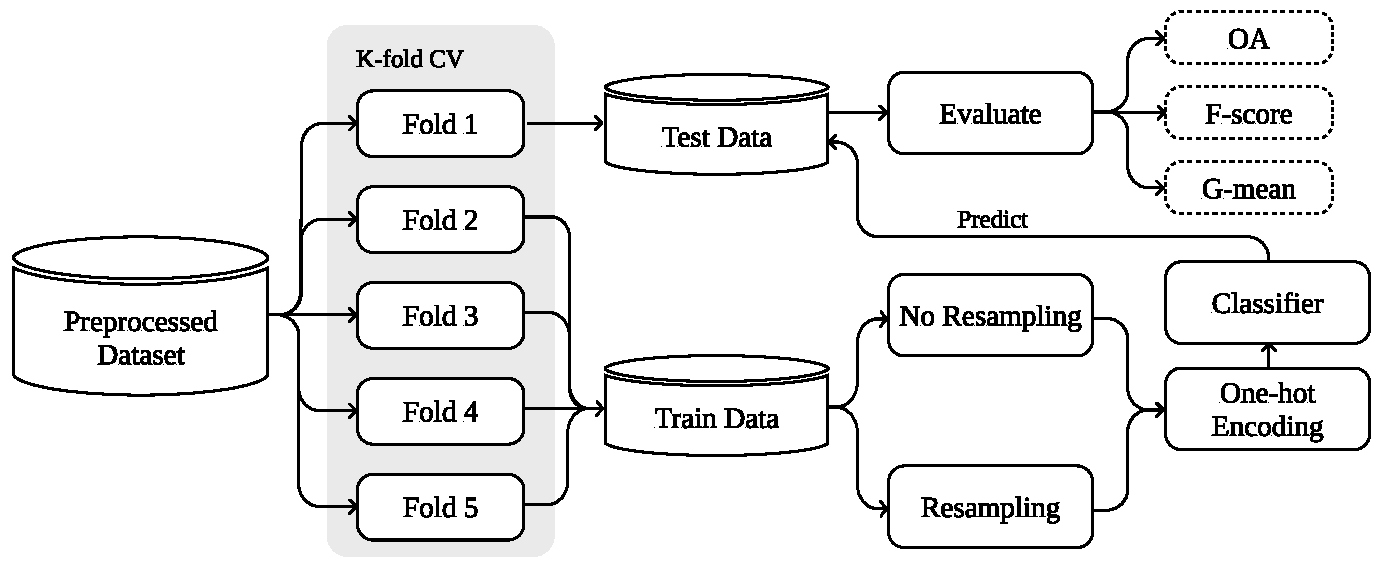
\includegraphics[width=.8\linewidth]{experimental_procedure}
    \caption{Experimental procedure used in this study.
    }~\label{fig:experimental_procedure-gsmotenc}
\end{figure}

A CV run consists of a stratified partitioning (\textit{i.e.}, each partition
contains the same relative frequencies of target labels) of the dataset into
five parts. A given resampler/classifier combination with a specific set of
hyperparameters is fit and tested five times, using one of the partitions as a
test set and the remaining ones as the training set. In the ML pipeline
defined for each run, the nominal features are one-hot encoded after
oversampling and before passing the data to the classifier. The estimated
performance consists of the average classification performance across the five
tests and three runs (\textit{i.e.}, a total of 15 tests). 

\subsection{Software Implementation}~\label{sec:software_implementation-gsmotenc}

The algorithmic implementation of G-SMOTENC was written using the Python
programming language and is available in the open-source package
\href{https://github.com/joaopfonseca/ml-research}{ML-Research}~\cite{Fonseca2021al},
along with other utilities used to produce the experiment and outputs used in
Section~\ref{sec:results_and_discussion-gsmotenc}. In addition, the packages
\href{https://github.com/scikit-learn/scikit-learn/}{Scikit-Learn}~\cite{Pedregosa2011},
\href{https://github.com/scikit-learn-contrib/imbalanced-learn}{Imbalanced-Learn}~\cite{JMLR:v18:16-365}
and \href{https://github.com/georgedouzas/research-learn/}{Research-Learn}
were also used in the experimental procedure to get the implementations of the
classifiers, benchmark over/undersamplers and run the experimental procedure.
The original SMOTE-ENC implementation was retrieved from the
\href{https://github.com/Mimimkh/SMOTE-ENC-code}{authors' GitHub repository}.
The Latex code, Python scripts (including data pulling and preprocessing,
experiment setup and analysis of results), as well as the datasets used, are
available in this \href{https://github.com/joaopfonseca/publications}{GitHub
repository}.
 
\section{Results and Discussion}~\label{sec:results_and_discussion-gsmotenc}

In this section, we present the experimental results. We focus on the
comparison of classification performance using oversamplers whose generation
mechanism is compatible with datasets containing both nominal and continuous
features. The experimental results were analyzed in two stages: (1) in
Section~\ref{sec:results-gsmotenc} we analyze mean rankings and absolute performances
and in Section~\ref{sec:statistical_analysis-gsmotenc} we show the results of our
statistical analysis. Section~\ref{sec:discussion-gsmotenc} discusses the main
insights extracted by analyzing the experimental results.

\subsection{Results}~\label{sec:results-gsmotenc}

Table~\ref{tbl:mean_sem_ranks} presents the mean rankings of CV scores between
the different combinations of oversamplers, metrics and classifiers. These
results were calculated by assigning a ranking score for each oversampler from
1 (best) to 4 (worst) for each dataset, metric and classifier.

\begingroup\small
{\setlength{\tabcolsep}{5pt}
\begin{longtable}{cccccccc}
\caption{Mean rankings over the different datasets, folds and runs used in the experiment.}
\label{tbl:mean_sem_ranks}\\
\toprule
Classifier &  Metric &                G-SMOTENC &                     NONE &         SMOTENC &                      ROS &             RUS &       SMOTE-ENC \\
\midrule
\endfirsthead
\caption[]{Mean rankings over the different datasets, folds and runs used in the experiment.} \\
\toprule
Classifier &  Metric &                G-SMOTENC &                     NONE &         SMOTENC &                      ROS &             RUS &       SMOTE-ENC \\
\midrule
\endhead
\midrule
\multicolumn{8}{r}{{Continued on next page}} \\
\midrule
\endfoot

\bottomrule
\endlastfoot
        DT &      OA &          1.66 $\pm$ 0.13 & \textbf{1.61 $\pm$ 0.27} & 3.58 $\pm$ 0.20 &          4.68 $\pm$ 0.15 & 5.42 $\pm$ 0.27 & 4.05 $\pm$ 0.23 \\
        DT & F-Score & \textbf{1.32 $\pm$ 0.11} &          3.84 $\pm$ 0.40 & 3.13 $\pm$ 0.20 &          4.32 $\pm$ 0.19 & 5.47 $\pm$ 0.23 & 2.92 $\pm$ 0.34 \\
        DT &  G-Mean & \textbf{1.68 $\pm$ 0.24} &          5.84 $\pm$ 0.09 & 2.82 $\pm$ 0.21 &          2.95 $\pm$ 0.32 & 4.26 $\pm$ 0.32 & 3.45 $\pm$ 0.30 \\
       KNN &      OA &          2.50 $\pm$ 0.17 & \textbf{1.37 $\pm$ 0.28} & 4.21 $\pm$ 0.25 &          3.34 $\pm$ 0.35 & 5.68 $\pm$ 0.22 & 3.89 $\pm$ 0.15 \\
       KNN & F-Score & \textbf{1.37 $\pm$ 0.16} &          3.95 $\pm$ 0.35 & 3.11 $\pm$ 0.29 &          3.47 $\pm$ 0.36 & 5.53 $\pm$ 0.23 & 3.58 $\pm$ 0.23 \\
       KNN &  G-Mean & \textbf{1.74 $\pm$ 0.17} &          5.84 $\pm$ 0.12 & 2.89 $\pm$ 0.23 &          3.76 $\pm$ 0.33 & 3.00 $\pm$ 0.45 & 3.76 $\pm$ 0.23 \\
        LR &      OA &          2.74 $\pm$ 0.19 & \textbf{1.37 $\pm$ 0.28} & 3.08 $\pm$ 0.21 &          4.34 $\pm$ 0.30 & 5.74 $\pm$ 0.17 & 3.74 $\pm$ 0.28 \\
        LR & F-Score & \textbf{2.11 $\pm$ 0.24} &          4.53 $\pm$ 0.35 & 2.37 $\pm$ 0.28 &          3.47 $\pm$ 0.32 & 5.21 $\pm$ 0.27 & 3.32 $\pm$ 0.38 \\
        LR &  G-Mean &          2.13 $\pm$ 0.26 &          6.00 $\pm$ 0.00 & 3.61 $\pm$ 0.21 & \textbf{2.11 $\pm$ 0.23} & 3.32 $\pm$ 0.40 & 3.84 $\pm$ 0.28 \\
        RF &      OA &          1.82 $\pm$ 0.11 & \textbf{1.24 $\pm$ 0.09} & 3.97 $\pm$ 0.16 &          4.32 $\pm$ 0.21 & 5.92 $\pm$ 0.06 & 3.74 $\pm$ 0.22 \\
        RF & F-Score & \textbf{1.32 $\pm$ 0.13} &          5.05 $\pm$ 0.31 & 3.16 $\pm$ 0.22 &          3.05 $\pm$ 0.31 & 5.37 $\pm$ 0.14 & 3.05 $\pm$ 0.27 \\
        RF &  G-Mean & \textbf{1.68 $\pm$ 0.22} &          5.79 $\pm$ 0.21 & 3.26 $\pm$ 0.28 &          2.47 $\pm$ 0.30 & 3.89 $\pm$ 0.35 & 3.89 $\pm$ 0.19 \\
\end{longtable}

}
\endgroup

Table~\ref{tbl:mean_sem_scores} presents the mean CV scores. Except for the
OA metric, G-SMOTENC either outperformed or matched the remaining
oversamplers.

\begingroup\small
{\setlength{\tabcolsep}{4.8pt}
\begin{longtable}{cccccccc}
\caption{Mean scores over the different datasets, folds and runs used in the experiment}
\label{tbl:mean_sem_scores}\\
\toprule
Classifier &  Metric &                G-SMOTENC &                     NONE &                  SMOTENC &                      ROS &             RUS &       SMOTE-ENC \\
\midrule
\endfirsthead
\caption[]{Mean scores over the different datasets, folds and runs used in the experiment} \\
\toprule
Classifier &  Metric &                G-SMOTENC &                     NONE &                  SMOTENC &                      ROS &             RUS &       SMOTE-ENC \\
\midrule
\endhead
\midrule
\multicolumn{8}{r}{{Continued on next page}} \\
\midrule
\endfoot

\bottomrule
\endlastfoot
        DT &      OA &          0.74 $\pm$ 0.05 & \textbf{0.75 $\pm$ 0.04} &          0.68 $\pm$ 0.04 &          0.66 $\pm$ 0.04 & 0.58 $\pm$ 0.04 & 0.65 $\pm$ 0.04 \\
        DT & F-Score & \textbf{0.56 $\pm$ 0.04} &          0.52 $\pm$ 0.04 &          0.54 $\pm$ 0.04 &          0.52 $\pm$ 0.04 & 0.48 $\pm$ 0.04 & 0.51 $\pm$ 0.04 \\
        DT &  G-Mean & \textbf{0.69 $\pm$ 0.03} &          0.60 $\pm$ 0.02 &          0.68 $\pm$ 0.03 &          0.67 $\pm$ 0.03 & 0.65 $\pm$ 0.03 & 0.66 $\pm$ 0.03 \\
       KNN &      OA &          0.69 $\pm$ 0.04 & \textbf{0.73 $\pm$ 0.05} &          0.67 $\pm$ 0.04 &          0.69 $\pm$ 0.05 & 0.57 $\pm$ 0.04 & 0.68 $\pm$ 0.05 \\
       KNN & F-Score & \textbf{0.53 $\pm$ 0.04} &          0.50 $\pm$ 0.04 &          0.52 $\pm$ 0.04 &          0.52 $\pm$ 0.04 & 0.46 $\pm$ 0.04 & 0.51 $\pm$ 0.04 \\
       KNN &  G-Mean & \textbf{0.66 $\pm$ 0.03} &          0.58 $\pm$ 0.03 &          0.64 $\pm$ 0.03 &          0.62 $\pm$ 0.03 & 0.65 $\pm$ 0.03 & 0.63 $\pm$ 0.03 \\
        LR &      OA &          0.68 $\pm$ 0.05 & \textbf{0.75 $\pm$ 0.04} &          0.68 $\pm$ 0.05 &          0.66 $\pm$ 0.05 & 0.58 $\pm$ 0.04 & 0.67 $\pm$ 0.04 \\
        LR & F-Score & \textbf{0.54 $\pm$ 0.04} &          0.52 $\pm$ 0.04 & \textbf{0.54 $\pm$ 0.04} &          0.53 $\pm$ 0.04 & 0.48 $\pm$ 0.04 & 0.52 $\pm$ 0.04 \\
        LR &  G-Mean & \textbf{0.69 $\pm$ 0.02} &          0.60 $\pm$ 0.03 &          0.68 $\pm$ 0.02 & \textbf{0.69 $\pm$ 0.03} & 0.67 $\pm$ 0.03 & 0.67 $\pm$ 0.03 \\
        RF &      OA &          0.74 $\pm$ 0.04 & \textbf{0.76 $\pm$ 0.04} &          0.69 $\pm$ 0.04 &          0.69 $\pm$ 0.04 & 0.59 $\pm$ 0.04 & 0.68 $\pm$ 0.05 \\
        RF & F-Score & \textbf{0.57 $\pm$ 0.04} &          0.48 $\pm$ 0.04 &          0.55 $\pm$ 0.04 &          0.55 $\pm$ 0.04 & 0.49 $\pm$ 0.04 & 0.53 $\pm$ 0.04 \\
        RF &  G-Mean & \textbf{0.70 $\pm$ 0.02} &          0.57 $\pm$ 0.02 &          0.68 $\pm$ 0.03 &          0.69 $\pm$ 0.03 & 0.68 $\pm$ 0.03 & 0.68 $\pm$ 0.02 \\
\end{longtable}

}
\endgroup

\subsection{Statistical Analysis}~\label{sec:statistical_analysis-gsmotenc}

It is necessary to use methods that account for the multiple comparison
problem to conduct an appropriate statistical analysis in an experiment with
multiple datasets. Based on the recommendations found in~\cite{Demsar2006}, we
applied a Friedman test followed by a Holm-Bonferroni test for post-hoc
analysis.

In Section~\ref{sec:performance_metrics-gsmotenc} we explained that OA, although easily
interpretable, is not an appropriate performance metric for imbalanced
learning problems. Therefore, the statistical analysis was developed using the
two imbalance-appropriate metrics used in the study: F-Score and G-Mean. Based
on the Friedman test~\cite{Friedman1937}, there is a statistically
significant difference in performance across resampling methods. The results
of this test are shown in Table~\ref{tbl:friedman_test}. The null hypothesis
is rejected in all cases.

\begin{longtable}{cccc}
\caption{Results for the Friedman test. Statistical significance is tested at a level of $\alpha = 0.05$. The null hypothesis is that there is no difference in the classification outcome across resamplers.}
\label{tbl:friedman_test}\\
\toprule
Classifier &  Metric & p-value &  Significance \\
\midrule
\endfirsthead
\caption[]{Results for the Friedman test. Statistical significance is tested at a level of $\alpha = 0.05$. The null hypothesis is that there is no difference in the classification outcome across resamplers.} \\
\toprule
Classifier &  Metric & p-value &  Significance \\
\midrule
\endhead
\midrule
\multicolumn{4}{r}{{Continued on next page}} \\
\midrule
\endfoot

\bottomrule
\endlastfoot
        DT & F-Score & 2.2e-10 &          True \\
        DT &  G-Mean & 1.2e-10 &          True \\
       KNN & F-Score & 2.3e-09 &          True \\
       KNN &  G-Mean & 9.4e-10 &          True \\
        LR & F-Score & 2.1e-07 &          True \\
        LR &  G-Mean & 9.7e-11 &          True \\
        RF & F-Score & 8.5e-12 &          True \\
        RF &  G-Mean & 2.0e-10 &          True \\
\end{longtable}


We performed a Holm-Bonferroni test to understand whether the difference in
the performance of G-SMOTENC is statistically significant to the remaining
resampling methods. The results of this test are shown in
Table~\ref{tbl:holms_test}. The null hypothesis is rejected in 33 out of 40
trials.

\begin{longtable}{ccccccc}
\caption{Adjusted p-values using the Holm-Bonferroni test. Statistical significance is tested at a level of $\alpha = 0.05$. The null hypothesis is that the benchmark methods perform similarly to the control method (G-SMOTENC).}
\label{tbl:holms_test}\\
\toprule
Classifier &  Metric &               NONE &            SMOTENC &                ROS &                RUS &          SMOTE-ENC \\
\midrule
\endfirsthead
\caption[]{Adjusted p-values using the Holm-Bonferroni test. Statistical significance is tested at a level of $\alpha = 0.05$. The null hypothesis is that the benchmark methods perform similarly to the control method (G-SMOTENC).} \\
\toprule
Classifier &  Metric &               NONE &            SMOTENC &                ROS &                RUS &          SMOTE-ENC \\
\midrule
\endhead
\midrule
\multicolumn{7}{r}{{Continued on next page}} \\
\midrule
\endfoot

\bottomrule
\endlastfoot
        DT & F-Score & \textbf{{1.5e-04}} & \textbf{{1.5e-04}} & \textbf{{7.3e-06}} & \textbf{{1.2e-06}} &          {1.0e-01} \\
        DT &  G-Mean & \textbf{{5.6e-07}} & \textbf{{2.7e-03}} & \textbf{{2.8e-02}} & \textbf{{3.9e-04}} & \textbf{{2.3e-02}} \\
       KNN & F-Score & \textbf{{6.4e-04}} & \textbf{{2.2e-04}} & \textbf{{7.2e-04}} & \textbf{{6.4e-04}} & \textbf{{5.9e-06}} \\
       KNN &  G-Mean & \textbf{{1.6e-05}} & \textbf{{9.6e-03}} & \textbf{{6.5e-03}} &          {2.0e-01} & \textbf{{3.5e-03}} \\
        LR & F-Score & \textbf{{4.0e-03}} &          {6.1e-01} & \textbf{{9.2e-03}} & \textbf{{3.6e-04}} &          {5.6e-02} \\
        LR &  G-Mean & \textbf{{1.6e-07}} & \textbf{{4.0e-04}} &          {8.6e-01} &          {2.4e-01} & \textbf{{4.7e-03}} \\
        RF & F-Score & \textbf{{1.7e-06}} & \textbf{{2.4e-04}} & \textbf{{8.0e-03}} & \textbf{{1.7e-06}} & \textbf{{8.0e-03}} \\
        RF &  G-Mean & \textbf{{3.8e-06}} & \textbf{{8.8e-03}} &          {2.5e-01} & \textbf{{2.3e-02}} & \textbf{{1.7e-03}} \\
\end{longtable}


\subsection{Discussion}~\label{sec:discussion-gsmotenc}

The results reported in Section~\ref{sec:results-gsmotenc} show that G-SMOTENC
consistently outperforms the remaining oversampling approaches. Based on the
two metrics appropriate for imbalanced learning problems, G-Mean and F-Score,
in the average rankings shown in Table~\ref{tbl:mean_sem_ranks} G-SMOTENC was
only outperformed once by a small margin. Unlike the results reported
in~\cite{mukherjee2021smote}, SMOTE-ENC's performance was rarely superior to
SMOTENC's.

The relative difference in the classifiers' performance is better visible in
Table~\ref{tbl:mean_sem_scores}. Using an RF classifier, for example, the
impact of using G-SMOTENC compared to no oversampling improves, on average, 13
percentual points on G-mean and nine percentual points using F-Score. 

The difference in performance between oversamplers was found to be
statistically significant across classifiers and performance metrics in the
Friedman test. The p-values of this test are reported in
Table~\ref{tbl:friedman_test}. The superiority of G-SMOTENC was confirmed with
the results from the Holm-Bonferroni test shown in Table~\ref{tbl:holms_test}.
This test showed that G-SMOTENC outperformed with statistical significance the
remaining resamplers in 82.5\% of the comparisons done.

\begin{figure}[ht]
	\centering
	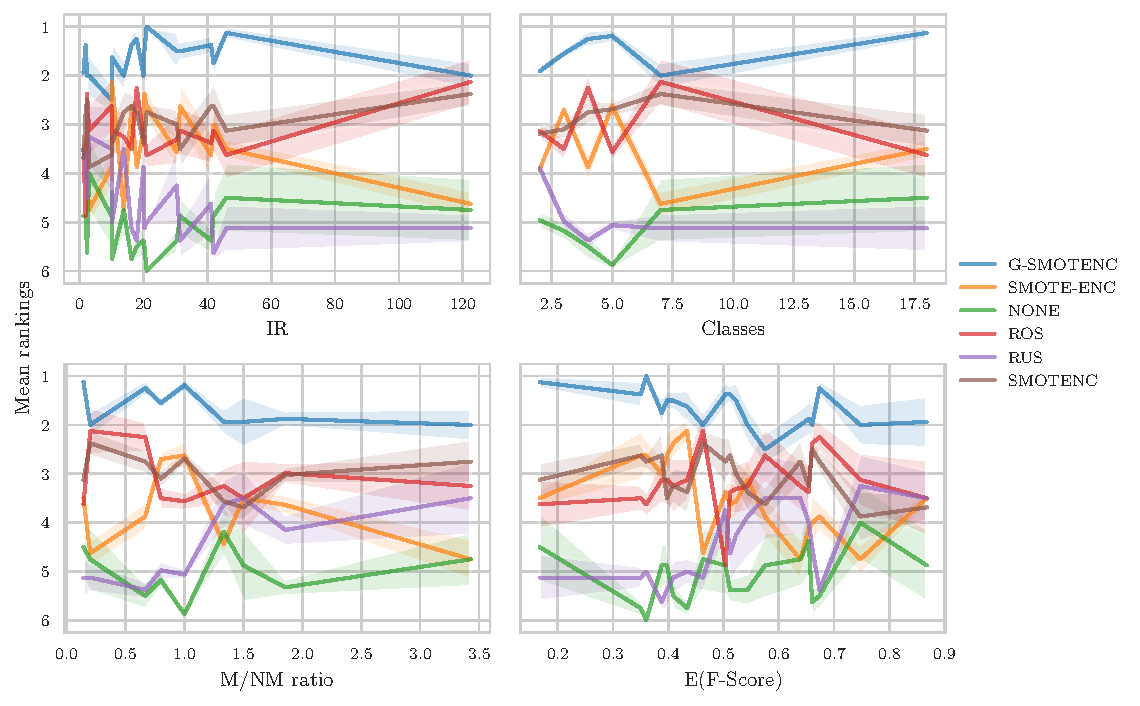
\includegraphics[width=\linewidth]{consistency_analysis_plot}
    \caption[Average ranking of oversamplers over different characteristics of
        the datasets used in the experiment.]{%
            Average ranking of oversamplers over different characteristics of
            the datasets used in the experiment. Legend: IR --- Imbalance
            Ratio, Classes --- Number of classes in the dataset, M/NM ratio
            --- ratio between the number of metric and non-metric features,
            E$($F-Score$)$ --- Mean F-Score of dataset across all combinations
            of classifiers and oversamplers.
    }~\label{fig:consistency_analysis}
\end{figure}


The results from this experiment expose some well-known limitations of SMOTE,
which become particularly evident with SMOTENC. Specifically, the lack of
diversity in the generated data and, on some occasions, the near-duplication
of observations discussed in~\cite{Douzas2019} may be a possible
explanation for the performance of SMOTENC being comparable to ROS'
performance, visible in Figure~\ref{fig:consistency_analysis}. In this
figure, three groups of resampling methods with comparable performance are
visible: (1) G-SMOTENC, the top-performing method, (2) SMOTENC, ROS and
SMOTE-ENC, where SMOTE-ENC has the most inconsistent behavior and (3) RUS and
no oversampling, the worst-performing approaches. In addition, G-SMOTENC's
superiority seems invariable to the dataset's characteristics, with little
overlap with the remaining benchmark methods.

\section{Conclusion}~\label{sec:conclusion-gsmotenc}

This paper presented G-SMOTENC, a new oversampling algorithm that combines
G-SMOTE and SMOTENC. This oversampling algorithm leverages G-SMOTE's data
selection and generation mechanisms into datasets with mixed data types. This
was achieved by encoding and generating nominal feature values using SMOTENC's
approach. The quality of the data generated with G-SMOTENC was tested over 20
datasets with different imbalance ratios, metric/non-metric feature ratios
and number of classes. These results were compared to no oversampling,
SMOTENC, Random Oversampling, Random Undersampling and SMOTE-ENC using a
Decision Tree, K-Nearest Neighbors, Logistic Regression and Random Forest as
classifiers.

G-SMOTENC can be seen as a drop-in replacement of SMOTENC, since when
$\alpha_{trunc}=1$, $\alpha_{def}=1$ and $\alpha_{sel}=minority$, SMOTENC is
reproduced. G-SMOTENC has three additional hyperparameters that allow for
greater customization of the selection and generation mechanisms.  However,
determining the optimal parameters a priori (\textit{i.e.}, with reduced
parameter tuning) is a topic for future work.

The results show that G-SMOTENC performs significantly better when compared to
its more popular counterparts (SMOTENC, Random Oversampling and Random
Undersampling), as well as a recently proposed oversampling algorithm for
mixed data types (SMOTE-ENC). This performance improvement is related to
G-SMOTENC's selection mechanism, which finds a safer region for data
generation, along with its generation mechanism which increases the diversity
of the generated observations compared to SMOTENC. The G-SMOTENC
implementation used in this study is available in the
\href{https://github.com/joaopfonseca/ml-research}{open-source Python library
``ML-Research''} and is fully compatible with the Scikit-Learn ecosystem.
